\chapter{Requirement Elicitation}

\section{Domain Context}
With the increasing demand for accessible and efficient printing services among students on campus, the HCMUT Smart Printing Service (HCMUT$\_$SSPS) is designed to address these needs by offering a centralized and user-friendly printing solution. Traditionally, students had to leave the campus to reach printing shops, which can be both time-consuming and inconvenient, especially when tight schedules or emergency arises. On top of that, external services may not offer the flexibility when it comes to printing options. Therefore, HCMUT$\_$SSPS aims to tackle these problems by offering a seamless on-campus printing service where students can easily upload documents, configure print settings, and pick up their paperwork from nearby printers without leaving the university.

The HCMUT$\_$SSPS system is designed to address these issues by offering an all-in-one printing solution directly on campus, allowing students to upload documents, choose from a variety of print options, and select their nearest campus printer through a web-based or mobile interface. This further facilitate students to fully customize their print jobs according to their preferences. In other words, the service allows for a seamless printing experience without the hassle of third-party shops. Moreover, with multiple printers located across different campus buildings, students can easily find a printer near them. With this option, students can plan around their busy academic timetable.

Beyond convenience, the system enhances security by keeping sensitive information locally since students no longer need to share personal information with external printing services, the risk of data breaches is reduced. The authentication functionality also allows students to track their printing history, providing transparency and an easy way to track usage. This combination of convenience, highly customization and keeping confidential data locally makes HCMUT$\_$SSPS an invaluable resource for students, streamlining the printing process and integrating it into campus life

\section{Stakeholders and Needs}
\vspace{-0.2em}
\begin{enumerate}[label=\textbf{\arabic*}.]
    \item \textbf{Students}
    users of the printing services. They can send print request, upload docu ments and purchase additional papers.  Students need the service to be easy to use, accessible from all places and secured along with the ability to review printing history.  
    \item \textbf{Student Printing Service Officer (SPSO)}
    who is responsible for managing student printing activities. The SPSO needs to manage printer settings, track and log printing activities and useful management tools.
    \item \textbf{IT staff}
    who responsible for developing, maintaining and upgrading the system. They need to build and develop the service for the university. 
    \item \textbf{University Administators}
    who manages resources and online payments system like BKPay. They need to be able to allocate resources and monitor transaction effectively. 
\end{enumerate}

\section{Benefits of the System}

\begin{itemize}
    \item \textbf{Students}
    
    Because of the user-friendly interface and accessible service like a web page, students can save time, increasing their productivity and satisfactory. Students also can format the documents to match their requirements. 
    \item \textbf{SPSO}
    
    The SPSO will be able to manage printing resources and settings efficiently. They can also review detailed reports of students’ printing activities, leading to better operational insights.
    \item \textbf{IT staff}
    
    The IT department can enhance users’ satisfactory and generate economic benefits for the service providers.
    \item \textbf{University Administrators}
    
    They can get a higher reputation and better financial efficiency through streamlined payments. 
\end{itemize}

\section{Functional Requirements}
\textbf{For Students}
\begin{enumerate}
    \item Students have the ability to upload documents for printing.
    \item Students can select printers and printing options, such as page size, number of copies, etc.
    \item They can view their printing history and page balances.
    \item Ability to purchase additional pages through an online payment system.
    \item Students can observe the status of print jobs, including start and end times, so they can determine when their prints are ready.
\end{enumerate}
\textbf{For SPSO}
\begin{enumerate}
    \item Ability to add, enable, or disable printers.
    \item SPSO can configure system settings such as page quotas and file types.
    \item SPSO can track the printing logs of students.
    \item SPSO has access to monthly and annual reports and can view them at any time.
    \item SPSO can schedule default page quotas for students each semester.
\end{enumerate}
\textbf{For IT staff}
\begin{enumerate}
    \item IT staff must be able to monitor the system’s performance, including server status, network connectivity, and printer availability across campus in real-time.
    \item IT staff must be able to add, remove, or troubleshoot printers within the network to ensure they are correctly connected to the system and operating properly.
    \item IT staff can maintain the HCMUT\_SSO authentication system, ensuring that students and staff can securely log in to the system.
    \item IT staff can create backups of the system's data (e.g., printing logs, configurations, user data) and perform data recovery in case of a failure.
    \item IT staff should be able to access and review system logs to troubleshoot any issues (e.g., failed print jobs, server errors, user access problems) and take corrective actions when necessary.
\end{enumerate}
\newpage
\textbf{For University Administrators}
\begin{enumerate}
    \item They can view system usage reports, such as the number of pages used, student printing activities, or dates.
    \item They must be able to monitor financial transactions through BKPay services.
    \item They can configure the default number of pages allocated to each student.
    \item They also have access to printing logs and resource usage.
    \item They can define roles and permissions for users, such as students, SPSO, and IT staff, so that each person can perform certain actions.
\end{enumerate}

\section{Non-Functional Requirements}
\begin{enumerate}
    \item The system should be accessible on both web and mobile platforms.
    \item The system must ensure user authentication via HCMUT\_SSO and enable payments via BKPay services.
    \item The system should facilitate fast and efficient document upload and printing.
    \item The system should handle large numbers of students and printers efficiently, supporting up to 1000 concurrent requests.
    \item To protect users' privacy, the system must ensure data confidentiality for printing logs and payment details.
\end{enumerate}

\section{Use-case Diagrams}
\subsection{Use-case Diagram for the Whole System}
\begin{figure}[H]
    % \vspace{-0.5cm}
    \centering
    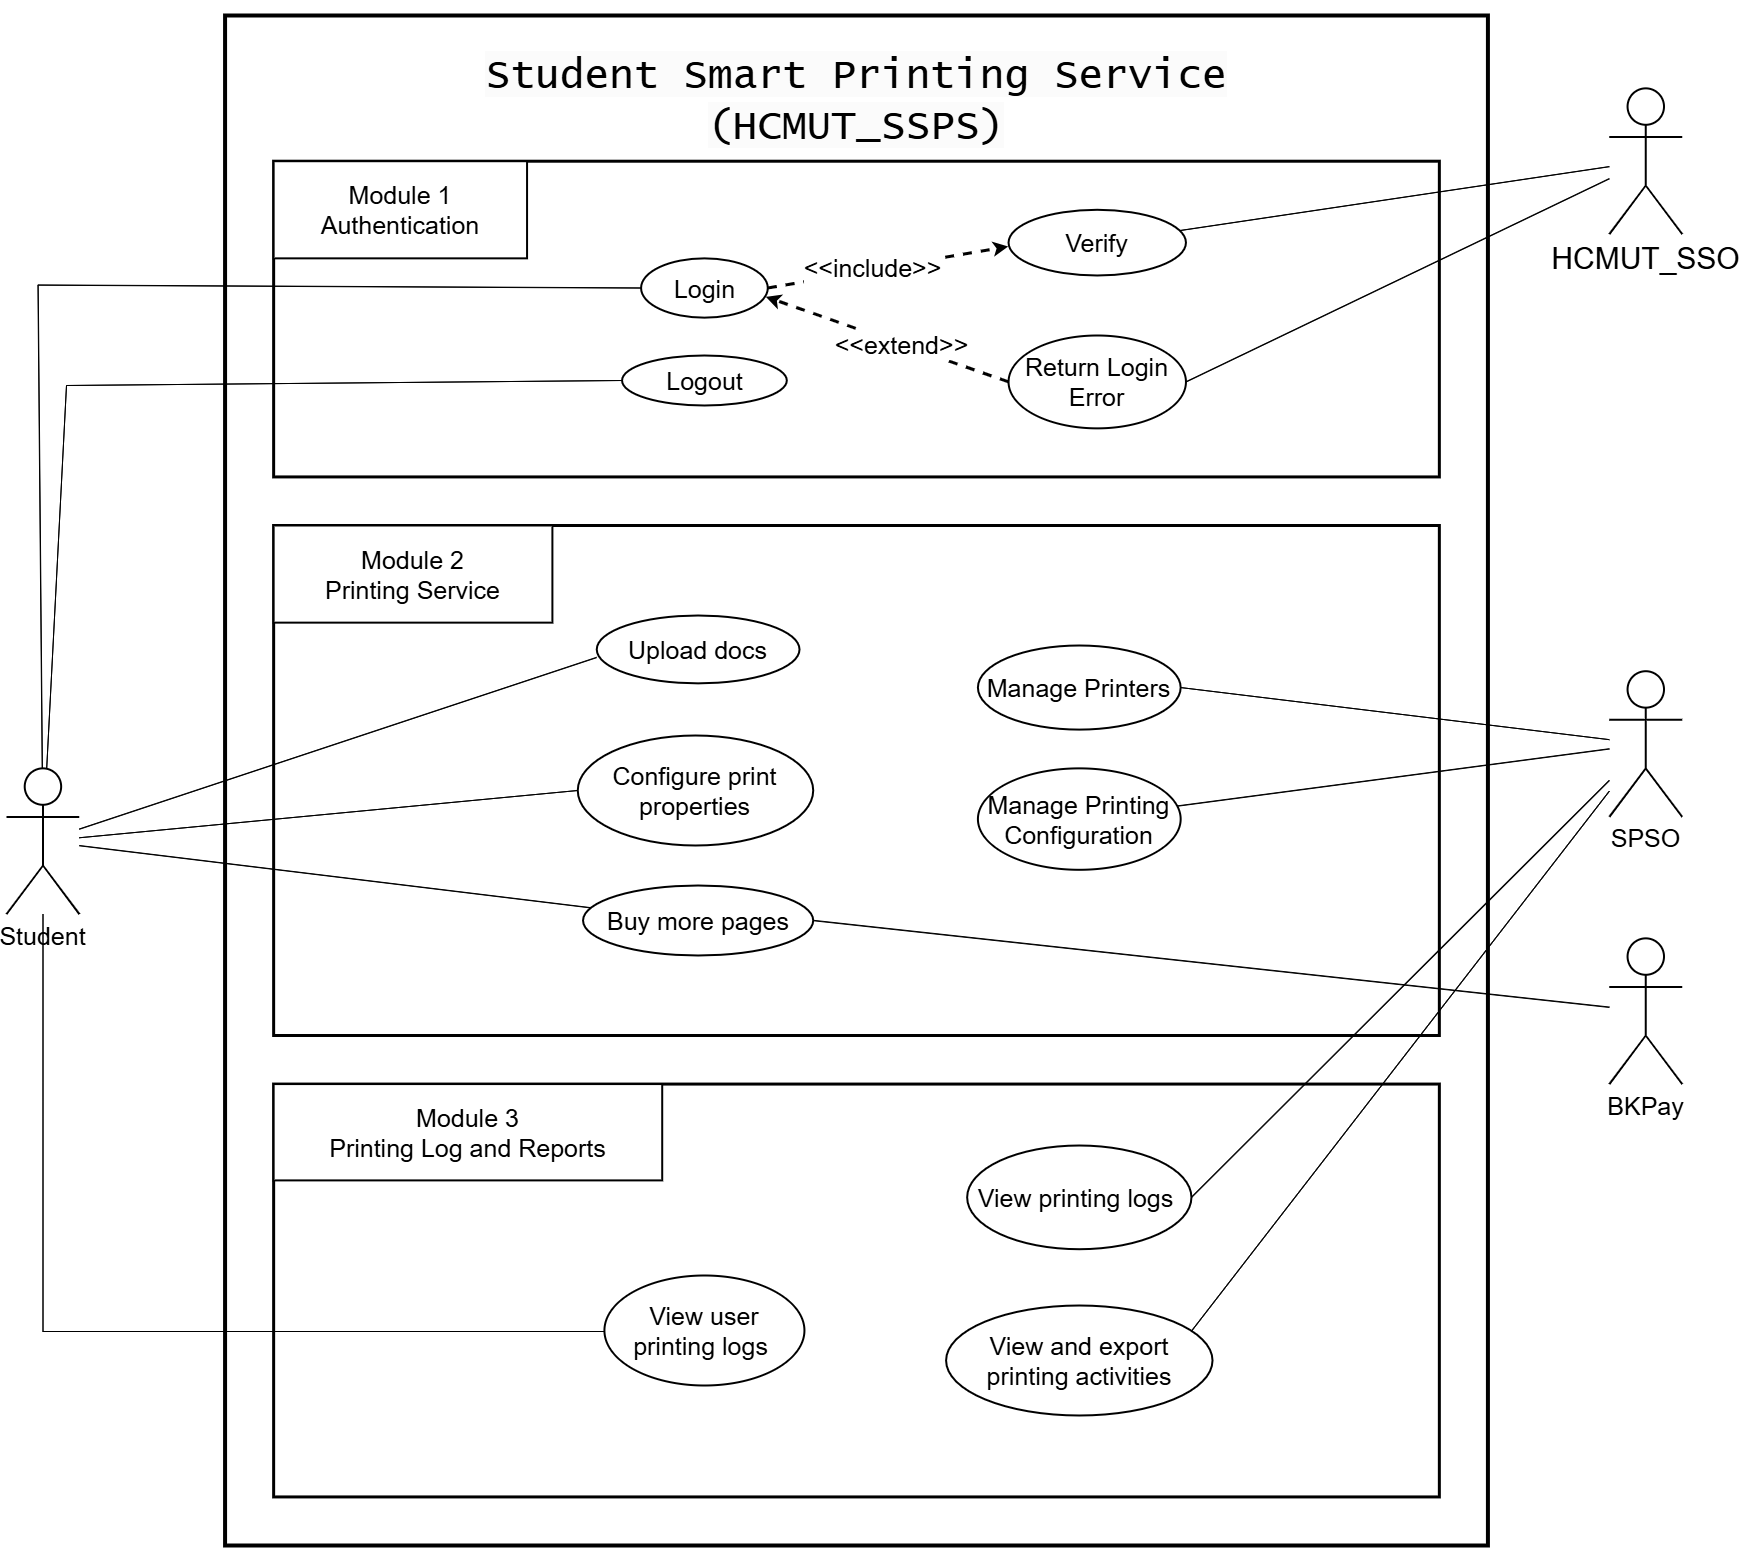
\includegraphics[width=\textwidth]{images/usecase_diagram/use_case_whole_system.png}
    \caption{Use-case Diagram for Whole System}
    \label{fig:use_case_whole_system}
\end{figure}

\clearpage
\begin{table}[h!]
\centering
\renewcommand{\arraystretch}{1.8}
% \small % Reduce font size for the table
\begin{tabular}{|>{\raggedright\arraybackslash}p{3cm}|>{\centering\arraybackslash}p{3cm}|p{7cm}|}
\hline
\textbf{Use Case Name} & \textbf{Actors} & \textbf{Description} \\ \hline
Login & Student,  HCMUT\_SSO & Allows the student to log in using HCMUT\_SSO authentication. \\ \hline
Logout & Student & Logs out the student from the system. \\ \hline
Upload Document & Student & Students upload documents to be printed by selecting a printer and configuring print properties. \\ \hline
Configure Print Properties & Student & Allows students to specify details like paper size, page range, and number of copies for printing. \\ \hline
Buy More Pages & Student, BKPay & Students purchase additional pages for printing by making a payment through BKPay. \\ \hline
View Printing Logs & Student, SPSO & Students and SPSO can view printing logs filtered by time period and printer. \\ \hline
Manage Printers & SPSO & SPSO can add, enable, or disable printers and modify printer configurations. \\ \hline
Manage Printing Configuration & SPSO & SPSO can manage settings like permitted file types and default page allocations. \\ \hline
View and Export Printing Activities & SPSO & SPSO can generate reports and export data on the usage of the printing service. \\ \hline
Authenticate Users & HCMUT\_SSO & HCMUT\_SSO authenticates students and SPSO before they can access the system. \\ \hline
Manage Page Quota & SPSO & SPSO can set default page quotas for students and update them during the semester. \\ \hline
Payment Processing & BKPay & Handles payment transactions for students purchasing more pages. \\ [2ex] \hline
\end{tabular}
\caption{Use-case Table for Whole System}
\label{tab:use_case_table_whole_system}
\end{table}




\subsection{Use-case Diagram for Printing Service Module}

\begin{figure}[H]
    % \vspace{-0.5cm}
    \centering
    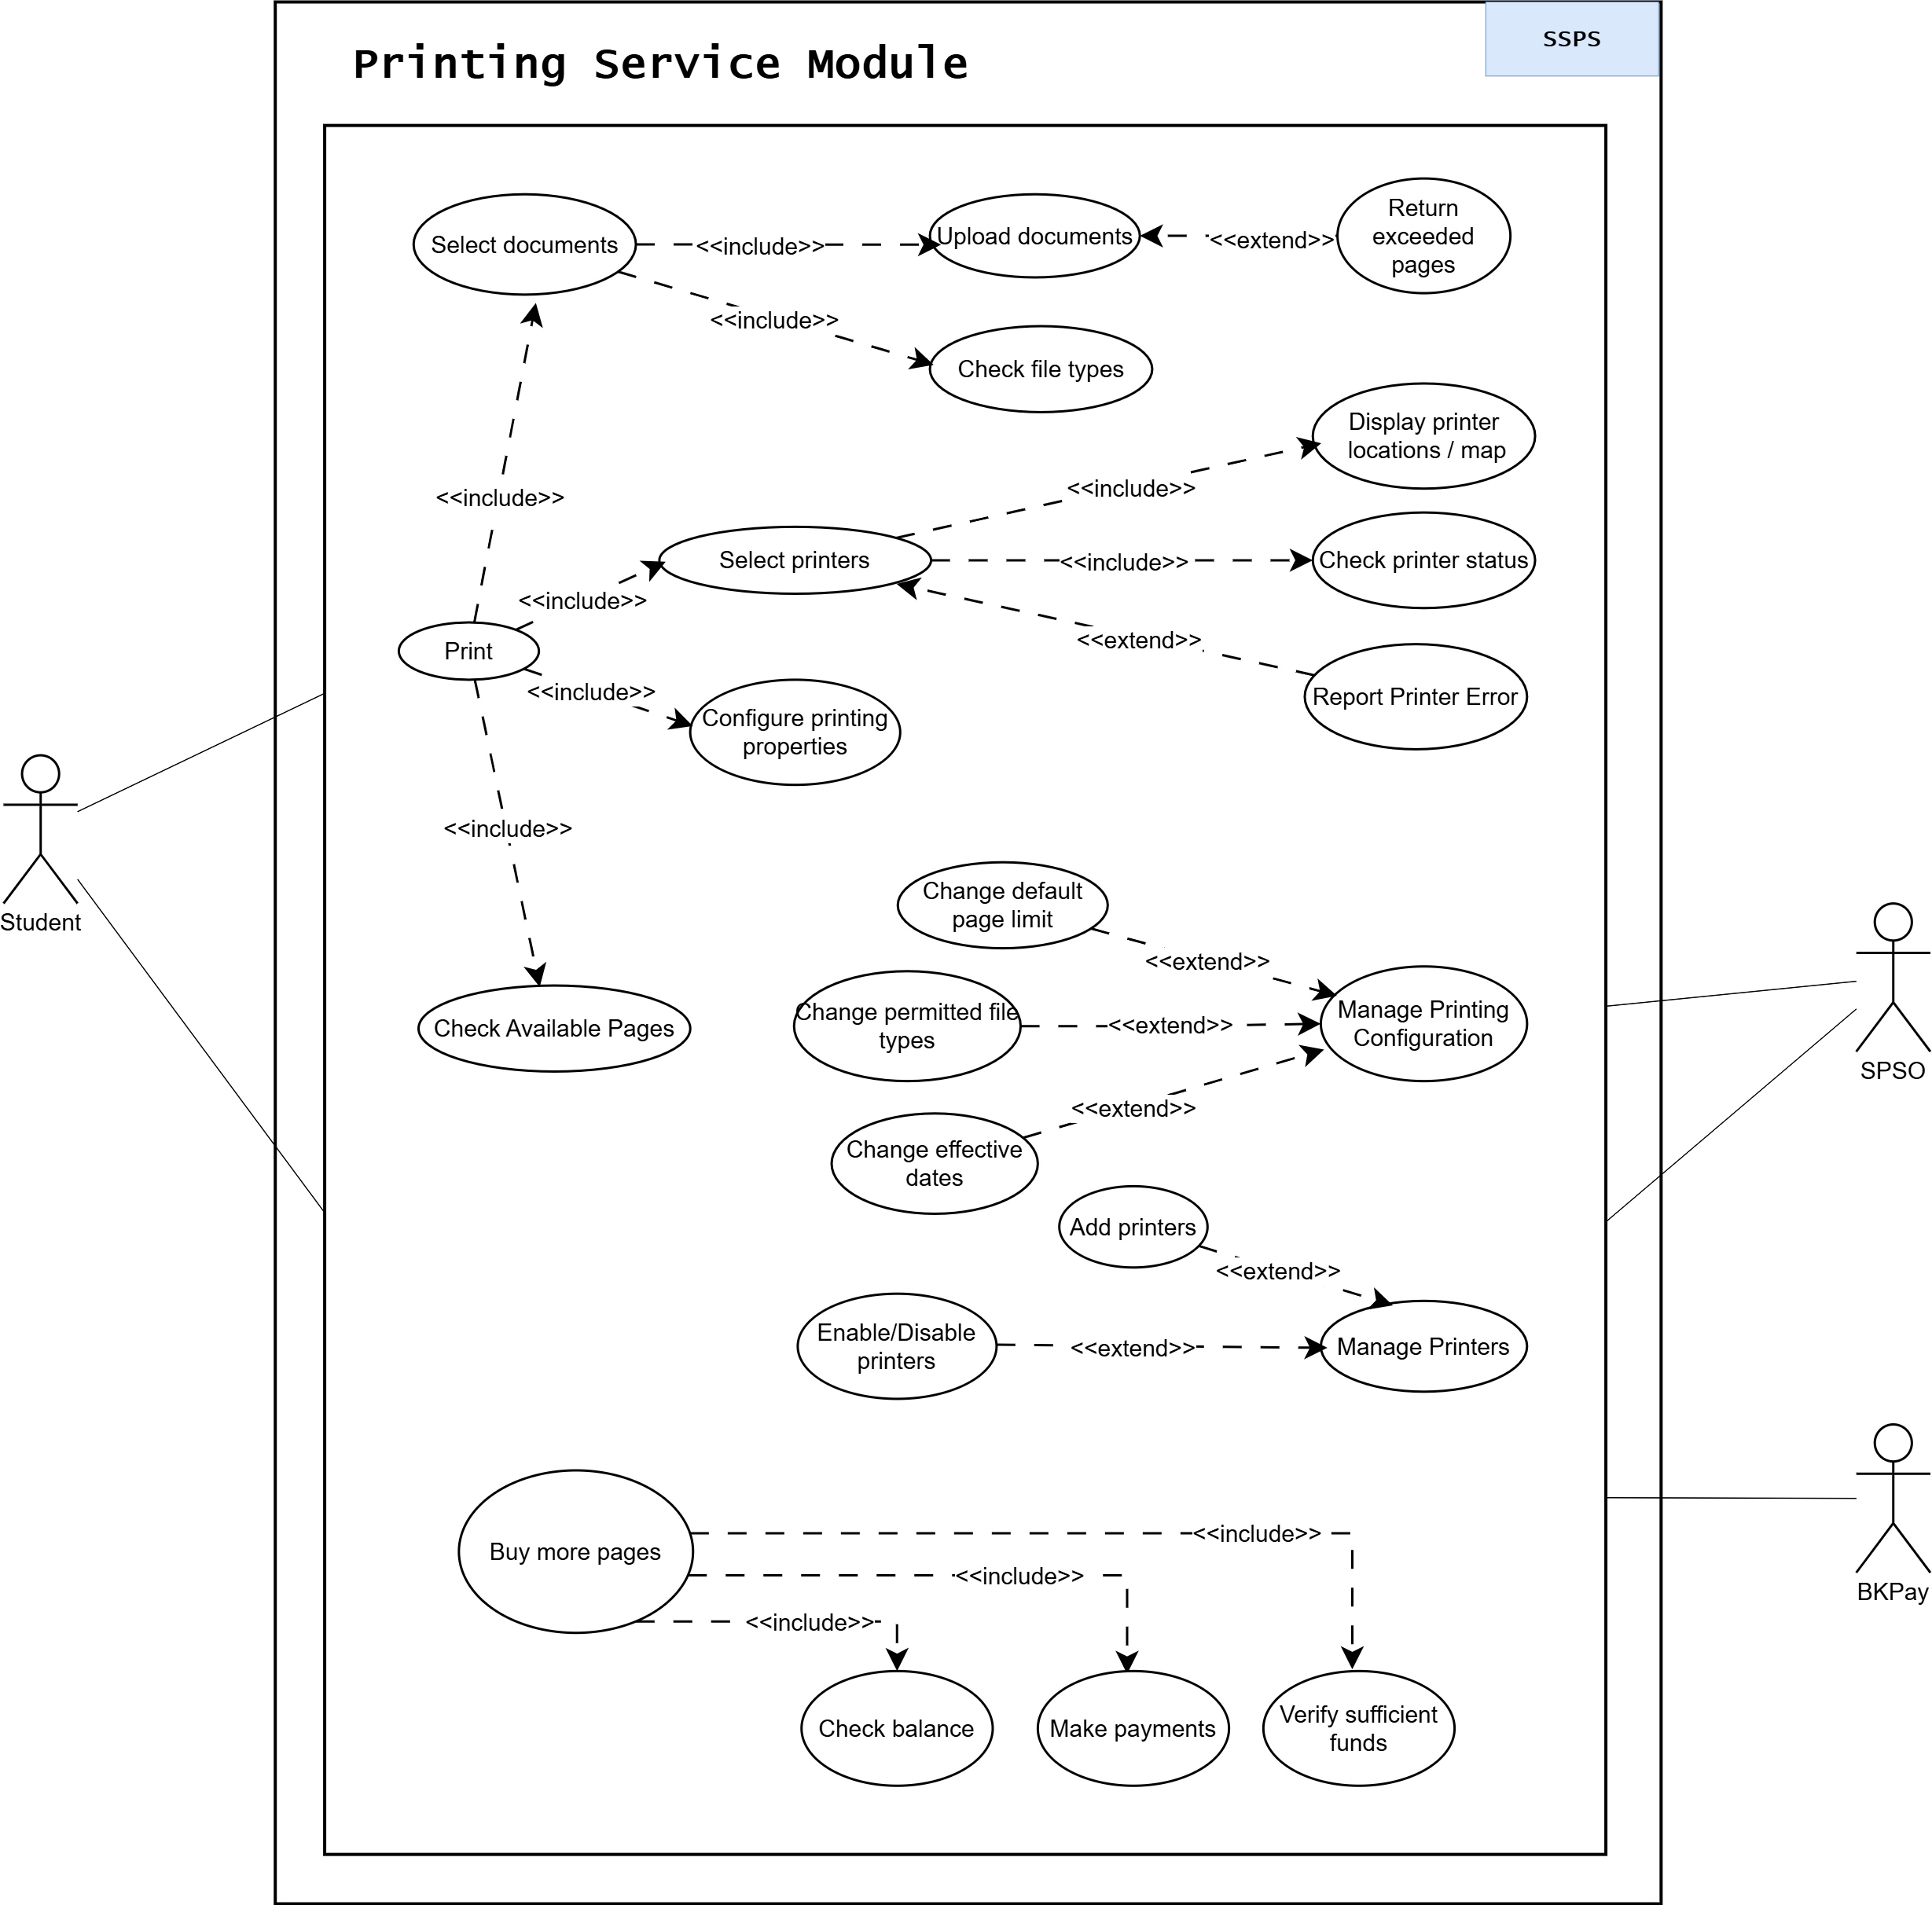
\includegraphics[width=\textwidth]{images/usecase_diagram/use_case_printing_service.png}
    \caption{Use-case Diagram for Printing Service Module}
    \label{fig:use_case_printing_service}
\end{figure}

\clearpage
\begin{table}[h!]
\centering
\renewcommand{\arraystretch}{1.8}
% \small % Reduce font size for the table
\begin{tabular}{|>{\raggedright\arraybackslash}p{3cm}|>{\centering\arraybackslash}p{3cm}|p{7cm}|}
\hline
\textbf{Use Case Name} & \textbf{Actors} & \textbf{Description} \\ \hline
Upload Documents & Student & The student uploads a document to be printed, and the system checks for supported file types. \\ \hline
Select Printer & Student & Allows the student to select a printer from a list or map based on availability. \\ \hline
Configure Printing Properties & Student & The student can configure the print job settings such as paper size, double-sided printing, and number of copies. \\ \hline
Print Documents & Student, Printer & The student sends the print job to the selected printer after configuring print settings. \\ \hline
Check Available Pages & Student & The system shows the student how many pages they can print based on their current balance. \\ \hline
Buy More Pages & Student, BKPay & The student buys additional printing pages by making a payment through BKPay. \\ \hline
Manage Printers & SPSO & The SPSO can add, enable, or disable printers, and check their statuses. \\ \hline
Manage Printing Configuration & SPSO & SPSO can change printing configurations such as default page limits, permitted file types, and effective dates. \\ \hline
Check Balance & Student, BKPay & Checks the student’s BKPay balance before making a payment for additional pages. \\ \hline
Make Payments & Student, BKPay & The student makes a payment for additional pages through BKPay. \\ \hline
Verify Sufficient Funds & BKPay & BKPay verifies that the student has sufficient funds to complete the payment for additional printing pages. \\ \hline
Return Exceeded Pages & System & If a student prints more pages than their balance allows, the system adjusts and refunds the exceeded portion. \\ \hline
Report Printer Error & Printer, System & If a printer encounters a technical problem (e.g., paper jam, out of ink), it reports the issue to the SPSO and the student. \\ [1ex] \hline
\end{tabular}
\caption{Use-case Table for Printing Service Module}
\label{tab:printing_service_use_case}
\end{table}

\newpage
\subsection{The Details of Usecases in Printing Service Module}

\begin{enumerate}\bfseries
    \item Usecase Login
    
       \begin{table}[h!]
        \centering
        \renewcommand{\arraystretch}{1.8}
        \begin{tabular}{|>{\centering\arraybackslash}m{3cm}|>{\raggedright\arraybackslash}m{10cm}|}
        \hline
        \textbf{Use Case Name} & Login \\ \hline
        \textbf{Actor(s)} & Student, HCMUT\_SSO \\ \hline
        \textbf{Description} & This use case describes the process by which a student logs into the system using their credentials. The student enters their username and password, and the system verifies these credentials via the HCMUT\_SSO service. Upon successful authentication, the student is granted access to the system’s features, such as uploading documents, viewing logs, and managing their printing account. \\ \hline
        \textbf{Preconditions} & The student must have valid login credentials. \\ \hline [2ex]
        \textbf{Basic Flow} &
        \begin{enumerate}
            \item The student selects the "Login" option.
            \item The system requests authentication details (username, password).
            \item The student enters their credentials.
            \item The system sends the credentials to HCMUT\_SSO for verification.
            \item HCMUT\_SSO verifies the credentials.
            \item The system logs the student in and grants access to printing services.
        \end{enumerate} \\ \hline
        \textbf{Alternative Flows} & If the credentials are incorrect, HCMUT\_SSO returns an error, and the system displays a "Login Error" message to the student. \\ \hline
        \textbf{Postconditions} & The student is logged in and can access the system’s services. \\ \hline
        \textbf{Exceptions} & If the HCMUT\_SSO service is unavailable, the system displays an error message and prompts the student to retry later. \\ [2ex] \hline
        \end{tabular}
        \caption{Use-case Table for Use Case “Login”}
        \label{tab:login_use_case}
        \end{table}
    \newpage
    \item Usecase Upload Documents
    

    
        \begin{table}[h!]
            \centering
            \renewcommand{\arraystretch}{1.8}
            \begin{tabular}{|>{\centering\arraybackslash}m{3cm}|>{\raggedright\arraybackslash}m{10cm}|}
            \hline
            \textbf{Use Case Name} & Upload Document \\ \hline
            \textbf{Actor(s)} & Student \\ \hline
            \textbf{Description} & The student uploads a document, selects a printer, and configures print settings. The system verifies the file type and processes the document for printing. \\ \hline
            \textbf{Preconditions} & The student must be logged in. The printer must be available. \\ \hline
            \textbf{Basic Flow} & 
            \begin{enumerate}
                \item The student selects the "Upload Documents" option.
                \item The system presents a file upload interface.
                \item The student uploads a document.
                \item The system verifies the file format (supported file types only).
                \item The student selects the printer and configures print properties.
                \item The system processes the document and sends it to the printer.
            \end{enumerate} \\ [-2ex] \hline
            \textbf{Alternative Flows} & If the file format is not supported, the system displays an error message and prompts the student to upload a valid file. \\ \hline
            \textbf{Postconditions} & The document is uploaded and queued for printing. \\ \hline
            \textbf{Exceptions} & 
            \begin{enumerate}
                \item \textbf{Unsupported File Format:} The system checks the document's file type and finds it unsupported (e.g., not PDF, DOCX). The system displays an error message: "Unsupported file format. Please upload a document in a supported format (PDF, DOCX, etc.)." The student is prompted to upload a valid file type.
                \item \textbf{File Size Too Large:} The system checks the file size and finds it exceeds the allowed limit. The system displays an error message: "File size too large. Please upload a file smaller than X MB." The student is prompted to upload a smaller file.
                \item \textbf{Network Issues:} The system detects network problems during the file upload. It displays an error message: "Network error. Please check your connection and try again." The system prompts the student to retry once the connection is restored.
            \end{enumerate} \\ \hline
            \end{tabular}
            \caption{Use-case Table for Use Case “Upload Document”}
            \label{tab:upload_document_use_case}
        \end{table}

    \newpage
    \item Usecase Buy More Pages
    
        \begin{table}[h!]
            \centering
            \renewcommand{\arraystretch}{1.8}
            \begin{tabular}{|>{\centering\arraybackslash}m{3cm}|>{\raggedright\arraybackslash}m{10cm}|}
            \hline
            \textbf{Use Case Name} & Buy More Pages \\ \hline
            \textbf{Actor(s)} & Student, BKPay \\ \hline
            \textbf{Description} & The student purchases additional printing pages through BKPay, and the system updates their account. \\ \hline
            \textbf{Preconditions} & The student must be logged in. The printer must be available. \\ \hline
            \textbf{Basic Flow} & 
            \begin{enumerate}
                \item The student selects "Buy More Pages".
                \item The system shows available packages.
                \item The student selects a package.
                \item The system redirects to BKPay for payment.
                \item The student completes the payment.
                \item BKPay confirms the transaction, and the system credits the student's account.
            \end{enumerate} \\ \hline
            \textbf{Alternative Flows} & 
            If the payment fails:
            \begin{enumerate}
                \item The system notifies the student that the payment was unsuccessful.
                \item The system presents options to retry the payment or select a different payment method. The student can:
                \begin{itemize}
                    \item Retry the transaction with the same payment method.
                    \item Select a different payment method from their BKPay account (e.g., different credit card or bank account).
                \end{itemize}
                \item The student attempts the transaction again, either by retrying the original method or using the alternative method.
                \item If successful, BKPay confirms the payment, and the system credits the student's account with the additional pages.
                \item If the payment fails again, the student is prompted to contact support or try later.
            \end{enumerate} \\ \hline
            \textbf{Postconditions} & The student's account is updated with the additional pages. \\ \hline
            \textbf{Exceptions} & If BKPay is unavailable, the system displays an error and advises the student to try again later. \\ [2ex] \hline
            \end{tabular}
            \caption{Use-case Table for Use Case “Buy More Pages”}
            \label{tab:buy_more_pages_use_case}
        \end{table}

    \newpage
    \item Usecase Manage Printers
    
        \begin{table}[h!]
            \centering
            \renewcommand{\arraystretch}{1.8}
            \begin{tabular}{|>{\centering\arraybackslash}m{3cm}|>{\raggedright\arraybackslash}m{10cm}|}
            \hline
            \textbf{Use Case Name} & Manage Printers \\ \hline
            \textbf{Actor(s)} & SPSO (Student Printing Service Officer) \\ \hline
            \textbf{Description} & This use case allows the SPSO to manage the printers in the system. The SPSO can add new printers, enable or disable existing printers, and modify printer details. The system saves these changes and updates the printer configurations for use by students. \\ \hline
            \textbf{Preconditions} & The SPSO must be logged in with administrative privileges. \\ \hline
            \textbf{Basic Flow} & 
            \begin{enumerate}
                \item The SPSO selects the "Manage Printers" option.
                \item The system displays a list of available printers.
                \item The SPSO can add new printers, enable or disable existing printers, or edit printer details.
                \item The SPSO submits the changes.
                \item The system saves the changes and updates the printer configurations.
            \end{enumerate} \\ \hline
            \textbf{Alternative Flows} & 
            If the printer cannot be added due to incorrect details (e.g., invalid location or model number):
            \begin{enumerate}
                \item The system detects the error in the printer details and prevents the submission.
                \item The system displays an error message describing the problem (e.g., "Invalid model number or location").
                \item The SPSO is prompted to correct the printer details.
                \item The SPSO corrects the input and resubmits.
                \item The system verifies the new input and, if valid, saves the changes successfully.
            \end{enumerate} \\ \hline
            \textbf{Postconditions} & The printer configurations are updated in the system and are available for student use. \\ \hline
            \textbf{Exceptions} & If the system fails to update the printer list due to technical issues, the SPSO is notified to try again later. \\ [2ex] \hline
            \end{tabular}
            \caption{Use-case Table for Use Case “Manage Printers”}
            \label{tab:manage_printers_use_case}
        \end{table}

    \newpage
    \item Usecase View Printing Logs
        \begin{table}[h!]
            \centering
            \renewcommand{\arraystretch}{1.8}
            \begin{tabular}{|>{\centering\arraybackslash}m{3cm}|>{\raggedright\arraybackslash}m{10cm}|}
            \hline
            \textbf{Use Case Name} & View Printing Logs \\ \hline
            \textbf{Actor(s)} & Student, SPSO \\ \hline
            \textbf{Description} & This use case allows the user (either a student or SPSO) to view the printing logs. The user can filter logs by date range and printer, and the system provides a summary of the number of pages printed by paper size. \\ \hline
            \textbf{Preconditions} & The user (student or SPSO) must be logged in to the system. \\ \hline
            \textbf{Basic Flow} & 
            \begin{enumerate}
                \item The user selects the "View Printing Logs" option.
                \item The system displays a list of logs for the selected time.
                \item The user can filter the logs by date range and printer.
                \item The system provides a summary of the printed pages by size (e.g., A4, A3).
            \end{enumerate} \\ \hline
            \textbf{Alternative Flows} & 
            If no logs are found for the selected period:
            \begin{enumerate}
                \item The system checks if there are any printing logs for the chosen time period and printer.
                \item If no logs are available, the system displays a message: "No logs found for the selected time period."
                \item The user can adjust the filters or select a different time period or printer.
            \end{enumerate} \\ \hline
            \textbf{Postconditions} & The requested printing logs are displayed to the user, including a summary of the number of pages printed by size. \\ \hline
            \textbf{Exceptions} & If the system fails to retrieve the logs:
            \begin{enumerate}
                \item The system encounters a problem while trying to access the logs (e.g., database connection error).
                \item The system displays an error message: "Unable to retrieve logs at this time. Please try again later."
                \item The user is prevented from viewing logs until the issue is resolved.
            \end{enumerate} \\ \hline
            \end{tabular}
            \caption{Use-case Table for Use Case “View Printing Logs”}
            \label{tab:view_printing_logs_use_case}
        \end{table}
\end{enumerate}

\newpage